\documentclass[12pt]{article}

\usepackage{sbc-template}
\usepackage{graphicx,url}
\usepackage[utf8]{inputenc}
\usepackage[brazil]{babel}
\usepackage[hidelinks,hyperindex,breaklinks]{hyperref}
     
\sloppy

\title{Aplicação dos algoritmos de árvore de decisão e rede neural \textit{feed-forward} para a classificação de dados do jogo DotA2}

\author{Eduardo Gil S. Cardoso\inst{1}, Gabriela S. Maximino\inst{1}, Igor Matheus S. Moreira\inst{1}}


\address{Instituto de Ciências Exatas e Naturais -- Faculdade de Computação\\
  Universidade Federal do Pará -- Belém, PA -- Brasil
  \email{\{eduardo.gil.s.cardoso,gabriela.maximino,igor.moreira\}@icen.ufpa.br}
}

\begin{document} 

\maketitle

\begin{abstract}
  This article presents the application of the decision tree and feed-forward artificial neural network algorithms in a database containing information about DotA2 game matches, aiming at data classification. This report is part of the deliverable associated to the task proposed by professor Reginaldo Cordeiro dos Santos Filho for the Artificial Intelligence course, taught under the Computer Science Bachelor’s degree program at the Federal University of Pará.
\end{abstract}
     
\begin{resumo} 
  Este artigo apresenta a aplicação dos algoritmos de árvore de decisão e rede neural artificial \textit{feed-forward} em uma base de dados contendo informações sobre partidas do jogo DotA2, visando a classificação dos dados. Este trabalho é parte do entregável relativo à tarefa proposta pelo Prof. Dr. Reginaldo Cordeiro dos Santos Filho para a disciplina de Inteligência Artificial, ministrada sob o curso de Bacharelado em Ciência da Computação na Universidade Federal do Pará.
\end{resumo}


\section{Introdução}\label{sec:intro}
A descoberta de conhecimento em base de dados (\textit{Knowledge Discovery in Databases} ou KDD) é o processo de descoberta de padrões válidos, potencialmente úteis e entendíveis a partir de dados. De modo geral, o KDD divide-se em 5 etapas: seleção; pré-processamento; transformação; mineração de dados; e interpretação de resultados \cite{fayyad}. Na etapa de mineração de dados, tem-se diversas tarefas; dentre elas, a classificação, responsável por rotular os dados em classes previamente definidas.

Nesse contexto, o terceiro trabalho da disciplina Inteligência Artificial propõe a realização do KDD em uma base de dados qualquer advinda do site \textit{UCI Machine Learning Repository}, considerando a utilização dos algoritmos de árvore de decisão e rede neural artificial para a tarefa de classificação na etapa de mineração de dados. Para tal, foi escolhido um repositório contendo informações sobre partidas do jogo DotA2, cuja classificação tenta predizer qual time ganhou a partida.

Diante disso, este trabalho se divide da seguinte forma: a Seção \ref{sec:descricao} apresenta a descrição da base de dados selecionada; a Seção \ref{sec:metodologia} descreve o processo de realização do trabalho; a Seção \ref{sec:resultados} apresenta os resultados da aplicação dos algoritmos; a Seção \ref{sec:analise} apresenta a comparação entre os dois algoritmos; por fim, a Seção \ref{sec:conclusao} sintetiza o trabalho e apresenta as considerações finais.

\section{Descrição da base de dados}\label{sec:descricao}
A base de dados escolhida, denominada \textit{DotA2 Game Results}, contém informações de partidas do jogo \textit{Defense of the Ancients} (DotA) e foi retirada do site \textit{UCI Machine Learning Repository}. Nesse jogo, vários modos e tipos de jogo podem ser escolhidos. Em todos eles, duas equipes compostas por 5 jogadores batalham entre si com diferentes heróis (personagens). Sendo assim, essa base contém 102.944 instâncias e 117 atributos (1 variável a ser predita/116 variáveis independentes). Nesses atributos, tem-se:

\begin{itemize}
	\item{\textbf{Time vencedor:}} variável a ser predita. Representa qual dos dois times ganhou a partida (-1 ou 1);
	\item{\textbf{ID de Cluster:}} variável categórica que indica a região em que o jogador está jogando; 
	\item{\textbf{Modo de jogo:}} variável categórica que indica o modo de jogo. Exemplo: \textit{all pick};
	\item{\textbf{Tipo de jogo:}} variável categórica que indica o tipo de jogo. Exemplo: \textit{ranked};
	\item{\textbf{Herói \{0, 1, ..., 111, 112\}:}} esse atributo se espalha por 113 colunas (uma para cada herói do jogo) e indica quais dos heróis foram utilizados pelos times: -1 se um time utilizou o herói; 0 se nenhum dos times utilizou o herói; e 1 se o outro time utilizou o herói.
\end{itemize}

Além disso, essa base encontra-se dividida em dois arquivos: \texttt{dota2Train.csv} e \texttt{dota2Test.csv}. A divisão original feita entre treino e teste, contudo, foi 90\%-10\%, enquanto que o estipulado para este trabalho é um \textit{Holdout} 70\%-30\%. Dessa forma, foi necessária a realização de um pré-processamento, a ser explicado na Seção \ref{sec:metodologia}, para resolver esse e outros problemas encontrados na base. 

A princípio, este conjunto de dados aparenta ser um pouco escasso em características, uma vez que praticamente não descreve características relacionadas ao desempenho dos jogadores no jogo (basicamente, as únicas características que envolvem os jogadores são as dos heróis, que expõem se uma das equipes escolheu um dado herói ou não). Considerando que esse é um jogo em que a atuação dos jogadores é decisiva em termos de desfecho (e.g., através de acúmulo de ouro, compra de itens, assistências, assassinatos e mortes), tem-se que este conjunto de dados certamente não possui um quadro tão abrangente quanto deveria.

\section{Metodologia do trabalho}\label{sec:metodologia}
De modo geral, este trabalho se dividiu em quatro etapas: tratamento da base de dados; seleção de características; aplicação dos algoritmos; e escrita do artigo.

Conforme mencionado anteriormente, alguns problemas foram encontrados na base de dados original. Esses problemas são: o tamanho de um arquivo \texttt{.csv} é substancialmente maior do que poderia ser, comparando com um arquivo \texttt{.h5}, uma vez que não há compressão nele; a divisão entre treino e teste é de 90\%-10\%, ao invés de 70\%-30\%; a variável a ser predita está no mesmo arquivo que as variáveis independentes; e algumas colunas possuem sempre os mesmos valores, sendo irrelevantes e agravando o problema da dimensionalidade. Dessa forma, a base dados precisou ser tratada.

Inicialmente, os arquivos \texttt{.csv} foram concatenados, as colunas irrelevantes foram removidas e o arquivo foi salvo em formato \texttt{.h5}. Em seguida, a base foi dividida aplicando o \textit{Holdout} estratificado 70\%-30\%, conforme o estipulado para este trabalho. Por fim, foi realizada a codificação das três variáveis categóricas para versões \textit{target-encoded} utilizando o algoritmo \textit{\textbf{K}-Fold Target Encoding}, com o objetivo de melhorar o conjunto de dados aos olhos dos algoritmos a serem empregados.

Feito isso, foi realizada a seleção de características para tentar descobrir quais são os atributos melhor correlacionados com a variável a ser predita e reduzir a alta dimensionalidade da base. Uma vez que as implementações da árvore de decisão e da rede neural \textit{feed-forward} utilizadas neste trabalho provêm da biblioteca \texttt{scikit-learn}, as funções usadas para pontuar as caracterísitcas foram \textit{ANOVA F-value}, \textit{Mutual Information} e \textit{Decision-tree feature importance}, da mesma biblioteca.

No intuito de verificar qual dos classificadores de características teve o melhor desempenho e qual número de características deveria ser escolhido, vários modelos foram gerados para realizar a validação cruzada sobre o conjunto de treinamento usando o algoritmo \textit{Stratified \textbf{K}-Fold}. Com base nos resultados obtidos, nota-se que há uma diferença entre o número de características ótimo para cada algoritmo: enquanto a árvore de decisão deve aprender com 10 características, a rede neural deve aprender com 30, sendo para ambos os casos as características melhor correlacionadas com a variável a ser predita de acordo com o classificador \textit{ANOVA F-value}. Para melhor detalhamento, recomenda-se a leitura do Jupyter Notebook no repositório \textbf{\href{https://github.com/ygarasab/data-classification}{@ygarasab/data-classification}}.

Com os aspectos importantes dos modelos a serem construídos definidos, passou-se para a aplicação dos algoritmos. Inicialmente, foi criado um modelo \textit{baseline} no qual, devido ser uma classificação binária, sempre prevê o rótulo que mais aparece. Para fins de comparação, a acurácia desse modelo também foi calculada. Em seguida, os algoritmos de árvore de decisão e rede neural \textit{feed-forward} foram executados 10 vezes, sendo coletadas em cada execução as métricas para a base de treinamento, base de teste e base completa. Essas métricas são a matriz de confusão, a sensibilidade, a especificidade, as confiabilidades positiva e negativa e a acurácia, conforme estipulado para o trabalho. 
	
\section{Resultados}\label{sec:resultados}
Na etapa de seleção de características, foi constatado que as dez características melhor correlacionadas na \textit{ANOVA F-value} são basicamente as mesmas que na \textit{Mutual information}, sendo todas elas não categóricas (i.e., heróis). Por outro lado, na \textit{Decision-tree feature importance}, as variáveis categórias (i.e., ID de Cluster, Modo de jogo e Tipo de jogo) ocuparam as três primeiras posições. Frente a isso, surgiram as perguntas: qual dos três classificadores teria o melhor desempenho? qual número de características a ser utilizado seria o melhor?

Para responder a essas perguntas, foi necessário gerar vários modelos e realizar a validação cruzada deles. Utilizando o algoritmo \textit{Stratified \textbf{K}-Fold}, o conjunto de dados de treino foi dividido em 10 partes de forma que, a cada rodada, uma parte foi utilizada como teste e as outras nove como treino. Quanto aos números de características, os tamanhos 5, 10, 15, 20, 25, 30, 50, 75 e 114 (todas as características) foram utilizados. Sendo assim, se o tamanho selecionado for 15 e o classificador escolhido for o \textit{ANOVA F-value}, por exemplo, então as 15 características melhor correlacionadas de acordo com esse classificador serão escolhidas para compor o modelo, que será então validado de forma cruzada. A partir dessa validação, a acurácia e pontuação F1 médias foram obtidas, e uma pontuação final foi criada a partir da média das duas medidas citadas.

\begin{figure}[t!]
    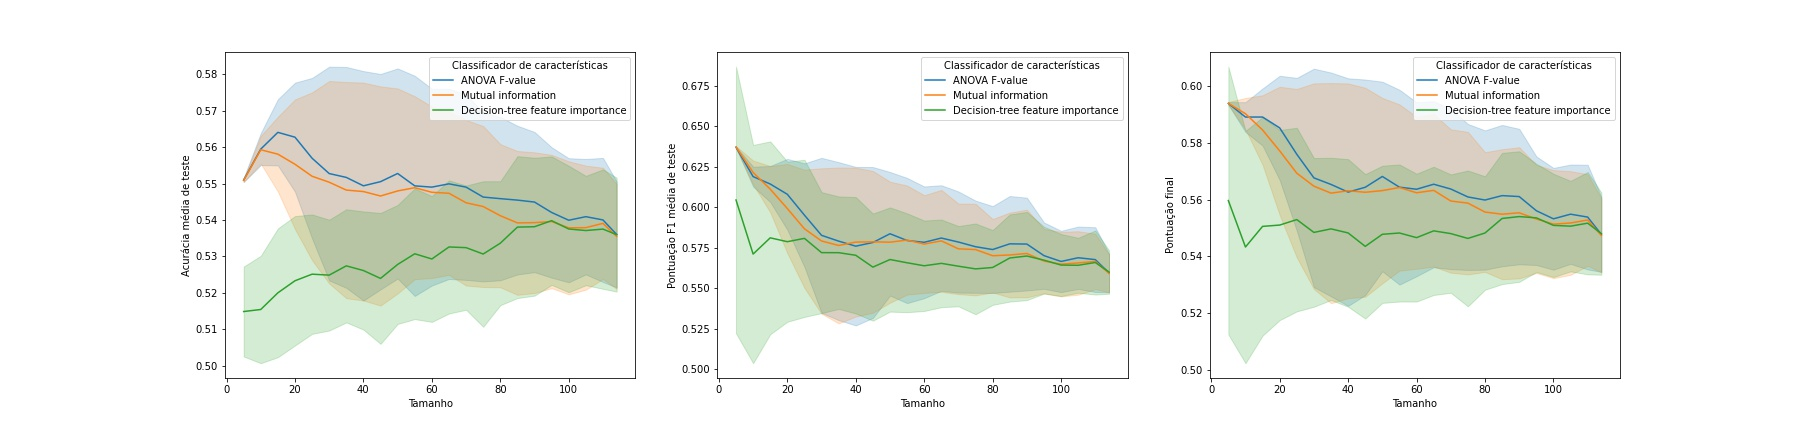
\includegraphics[width=\linewidth]{figures/modelos_por_classificador}
    \caption{Métricas dos modelos por classificador. Fonte: acervo próprio.}
    \label{fig:modelos-classif}
\end{figure}

Na \autoref{fig:modelos-classif} é possível observar como o aumento do número de características utilizadas impacta a acurácia, a pontuação F1 e a pontuação final (i.e., a média entre a acurácia e a pontuação F1) dos modelos resultantes. Nota-se que, com exceção do classificador \textit{Decision-tree feature importance}, a acurácia cai à médida em que o número de características aumenta. O comportamento desse classificador causa estranhamento, talvez indicando que ele não seja um bom estimador da correlação das características com os rótulos de classe.

\begin{figure}[t!]
    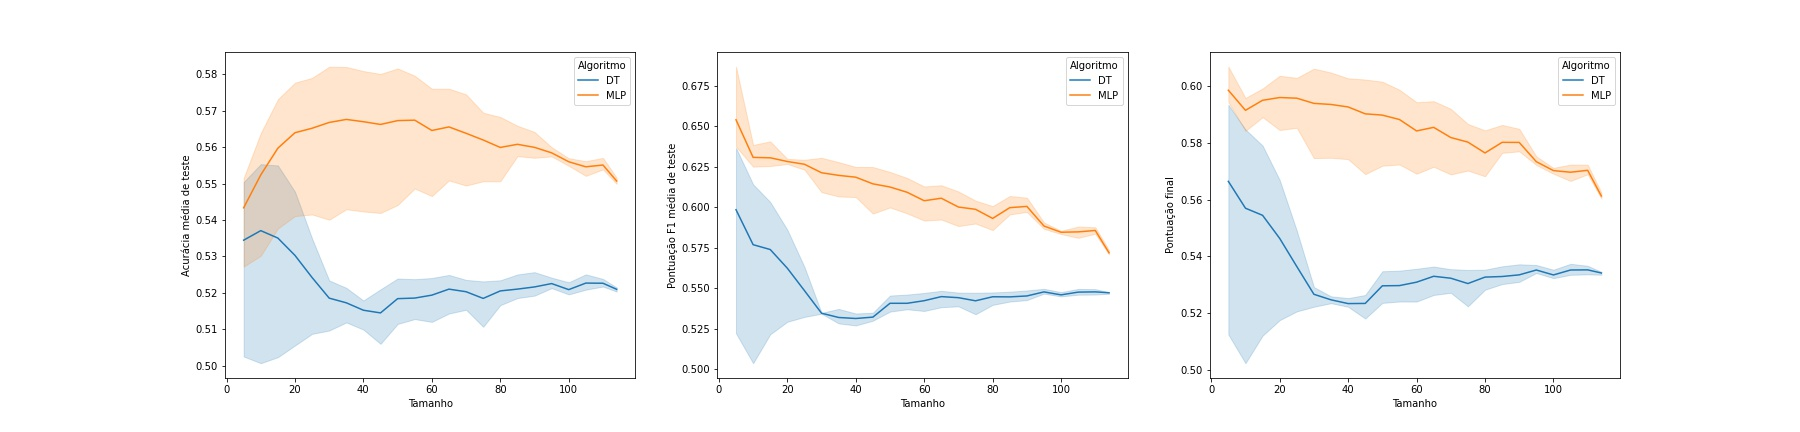
\includegraphics[width=\linewidth]{figures/modelos_por_algoritmo}
    \caption{Métricas dos modelos por algoritmo. Fonte: acervo próprio.}
    \label{fig:modelos-alg}
\end{figure}

Já na  \autoref{fig:modelos-alg}, que expõe as mesmas métricas da figura anterior só que agrupadas por algoritmo ao invés de classificador, é possível perceber que há números de características ótimos diferentes para cada algoritmo. Para a árvore de decisão, o melhor tamanho aparenta ser por volta de 10. No caso da rede neural, por volta de 30.

Finalizando a etapa de seleção de características, foi feita uma última análise acerca do tempo médio de treino dos algoritmos. Na  \autoref{fig:tempo-treino}, observa-se como o aumento no número de características impacta o tempo de treinamento da árvore de decisão (DT) e da rede neural (MLP). Com isso, tem-se que é muito mais custoso treinar uma rede neural do que uma árvore de decisão, conforme já esperado. 

\begin{figure}[t!]
    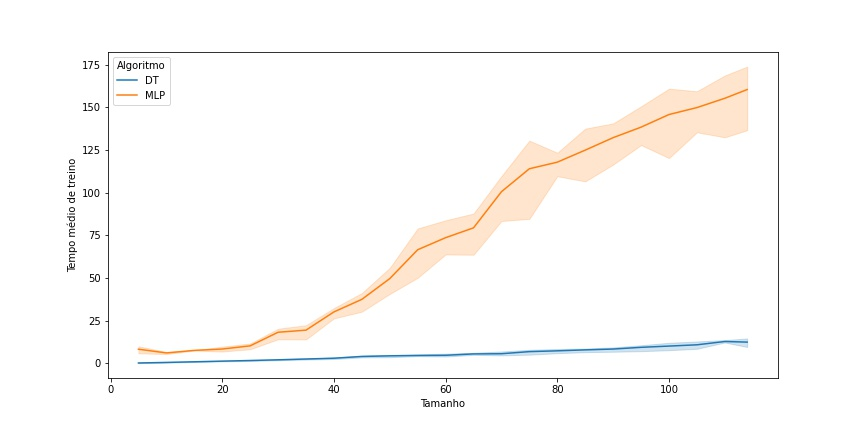
\includegraphics[width=\linewidth]{figures/tempo_treino}
    \caption{Tempo médio de treino para os algoritmos utilizados. Fonte: acervo próprio.}
    \label{fig:tempo-treino}
\end{figure}

Considerando as informações obtidas até o momento, as seguintes decisões foram feitas: o classificador \textit{ANOVA F-value} foi escolhido para ser utilizado; a rede neural utilizará as 30 características melhor correlacionadas; e a árvore de decisão utilizará as 10 características melhor correlacionadas.

Antes da aplicação dos algoritmos, contudo, foi necessário definir o valor da profundidade máxima da árvore de decisão. Nesse sentido, sabe-se que, com os valores-padrão da implementação do \texttt{scikit-learn} da árvore de decisão, há uma tendência que ocorra \textit{overfitting}. Isso foi constatado ao visualizar a árvore de decisão construída até o momento, conforme ilustra a \autoref{fig:arvore_padrao}, a qual possui 20 como valor padrão para a profundidade máxima.

\begin{figure}[t!]
    
\includegraphics[width=\linewidth]{figures/arvore_padrao}
    \caption{Árvore de decisão com profundidade máxima padrão. Fonte: acervo próprio.}
    \label{fig:arvore_padrao}
\end{figure}

No intuito de resolver esse problema, foram testadas todas as profundidades no intervalo [1, 20] de modo a visualizar como a acurácia, a pontuação F1 e a pontuação final resultante evoluem à medida em que o valor da profundidade máxima aumenta. A \autoref{fig:acuracia_profundidade} mostra os resultados obtidos. 

\begin{figure}[t!]
    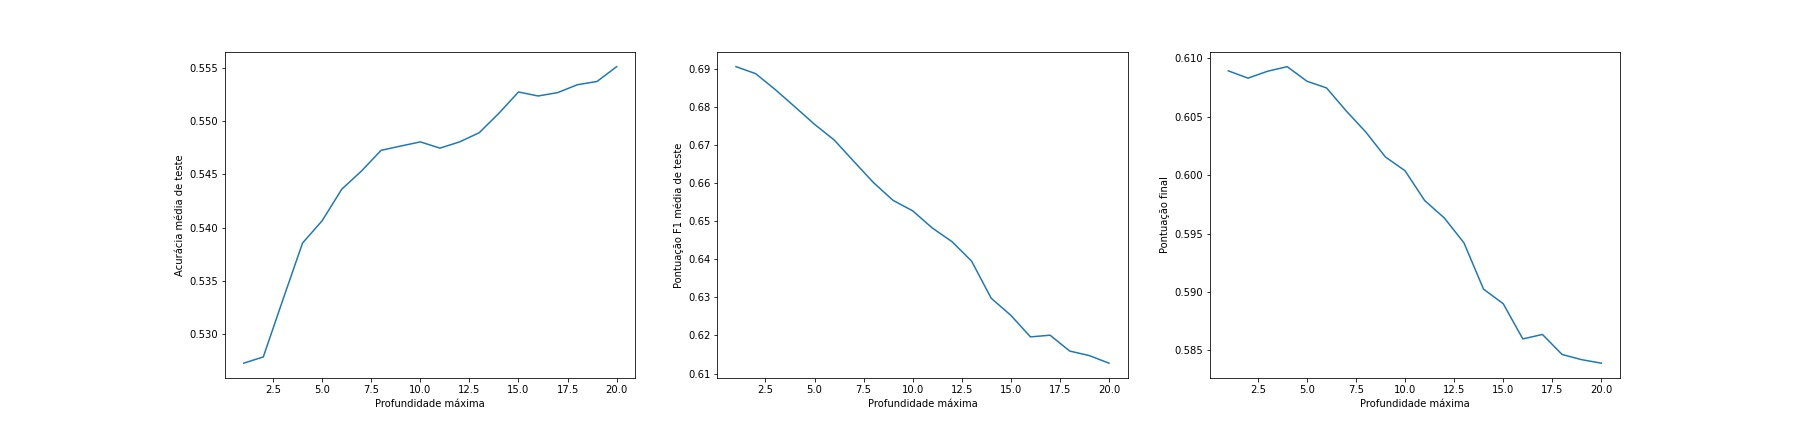
\includegraphics[width=\linewidth]{figures/acuracia_por_profundidade}
    \caption{Evolução das métricas da árvore por profundidade. Fonte: acervo próprio.}
    \label{fig:acuracia_profundidade}
\end{figure}

Testando a árvore quando a profundidade máxima é igual a 3, 5 e 7, obtém-se os resultados exibidos na \autoref{fig:arvore357}. Considerando o número de características (10), estipulou-se como razoável adotar a profundidade máxima da árvore como 3.

\begin{figure}[t!]
    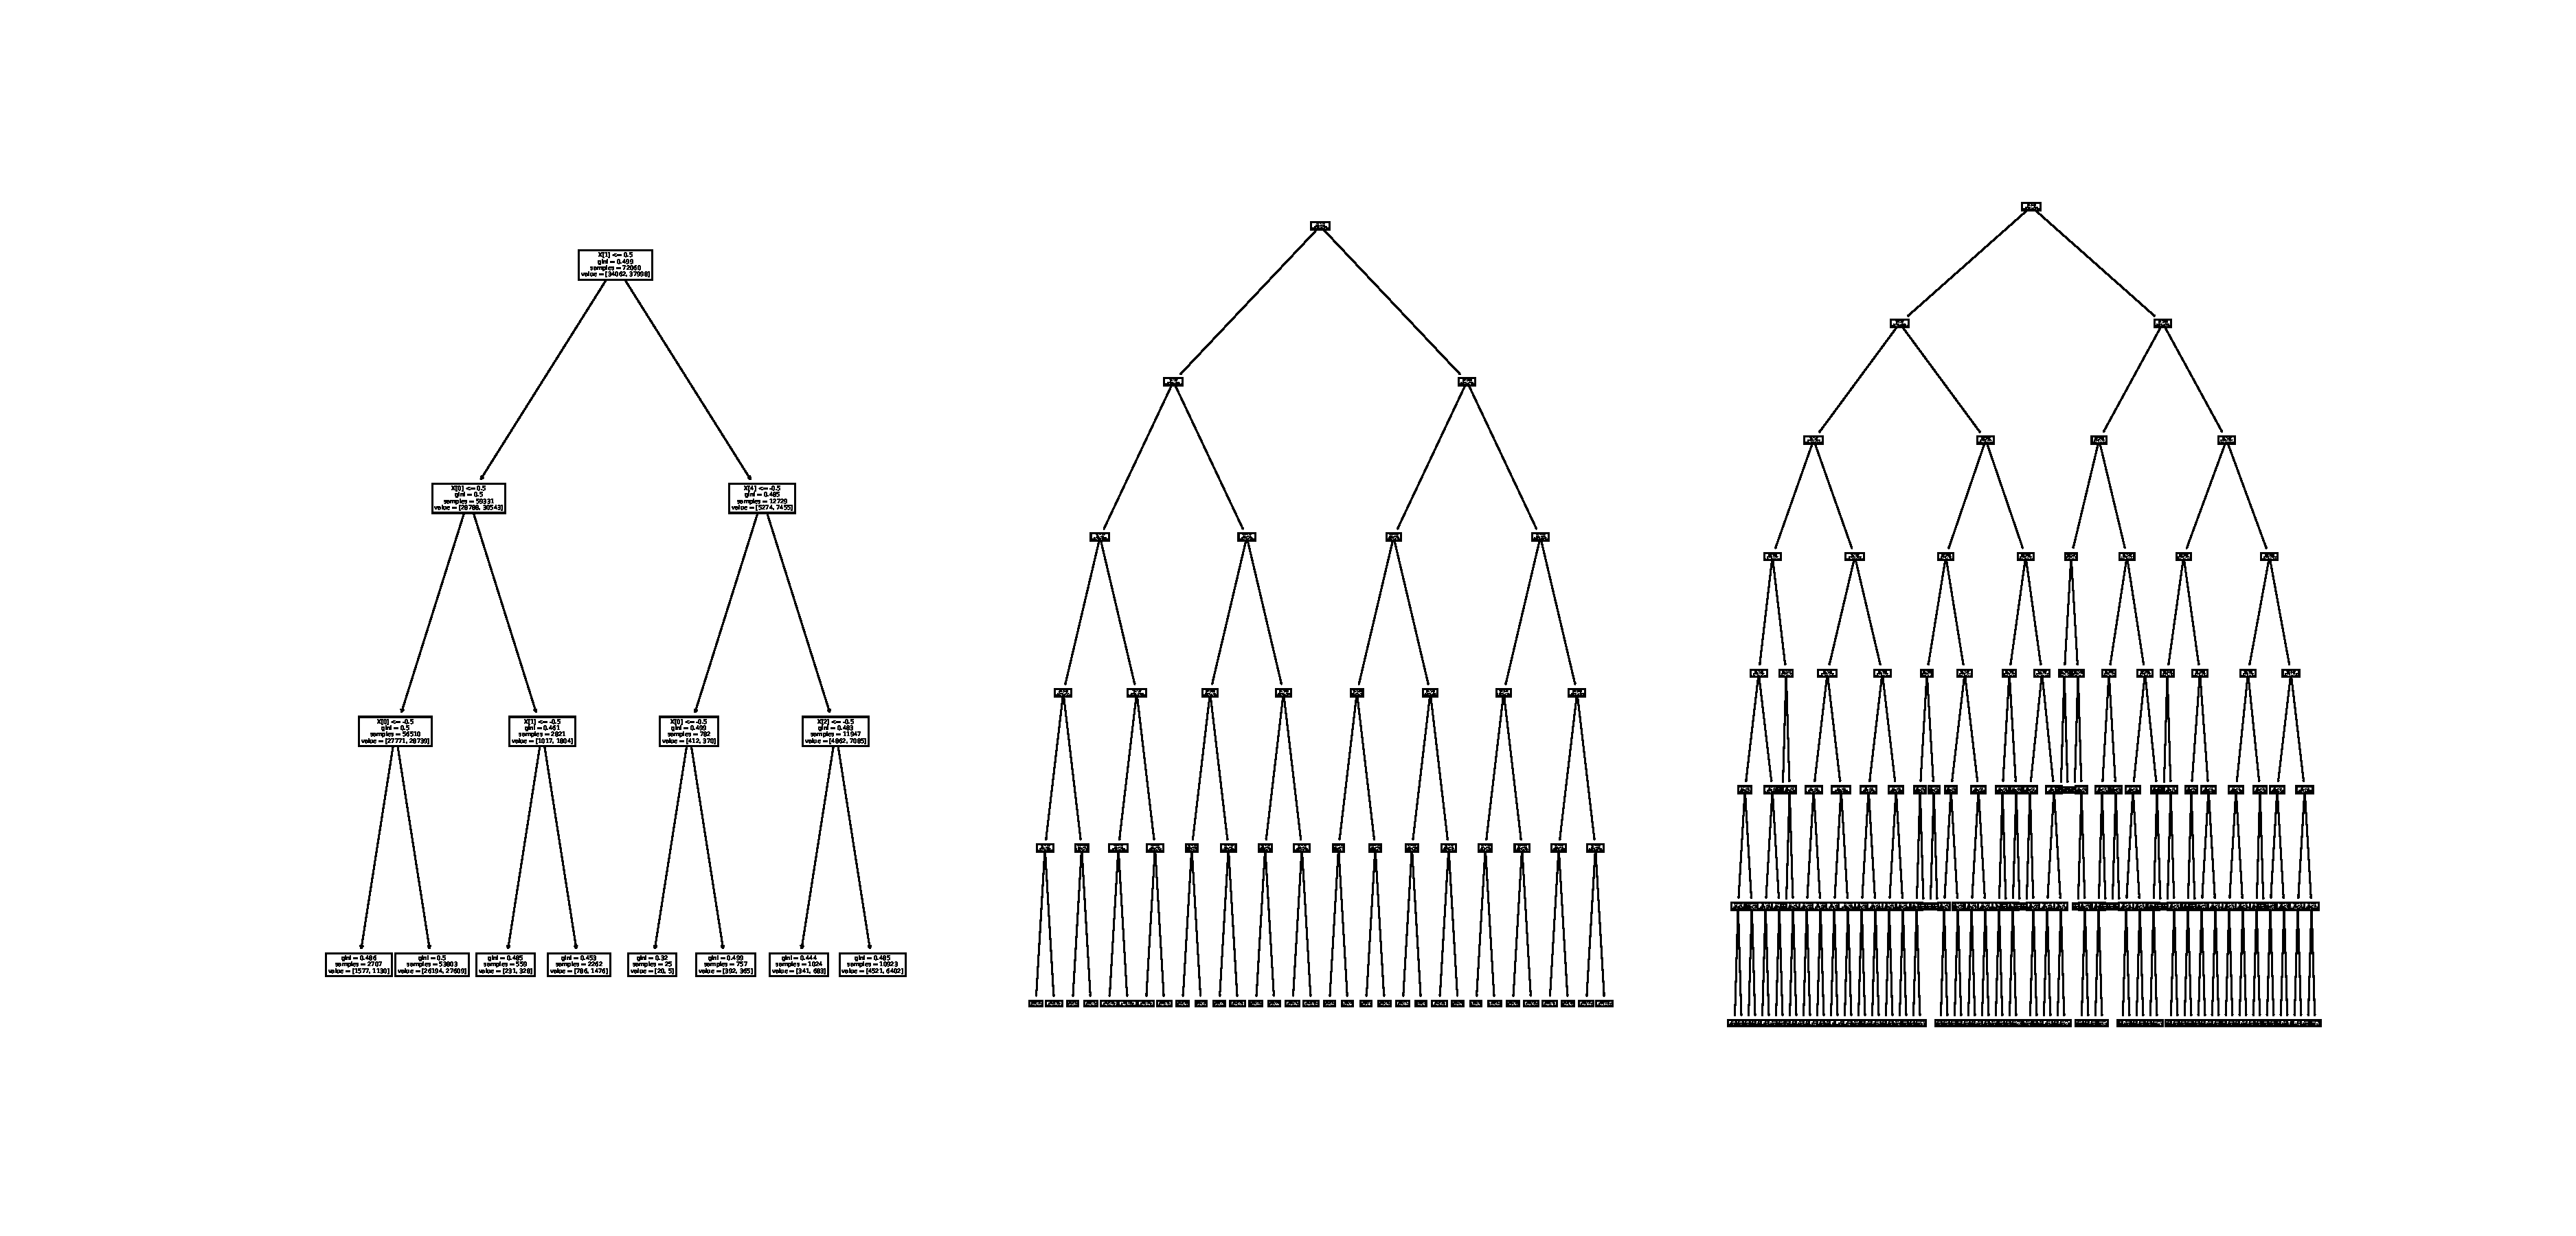
\includegraphics[width=\linewidth]{figures/arvore_357}
    \caption{Árvores de decisão com profundidade máxima 3, 5 e 7, respectivamente. Fonte: acervo próprio.}
    \label{fig:arvore357}
\end{figure}

Já na etapa de aplicação dos algoritmos, inicialmente foi criado um modelo \textit{baseline} para fins de comparação com os algoritmos a serem utilizados. Como no caso em questão tem-se uma classificação binária, o modelo \textit{baseline} para este conjunto de dados seria prever sempre o rótulo que mais aparece. Dessa forma, a acurácia-base do modelo construído foi de 52,7\%.

Em seguida, os algoritmos foram aplicados, sendo executados 10 vezes cada. As métricas coletadas para cada execução, conforme pedido para este trabalho, foram a matriz de confusão, sensibilidade, especificidade, confiabilidade positiva, confiabilidade negativa e acurácia. A tabela contendo esses resultados pode ser encontrada no Jupyter Notebook no repositório \textbf{\href{https://github.com/ygarasab/data-classification}{@ygarasab/data-classification}}.

Por fim, foram calculados a média e o desvio padrão da acurácia total do conjunto de modelos construídos para cada algoritmo, que estão ilustrados na \autoref{fig:resultados}.

\begin{figure}[t!]
    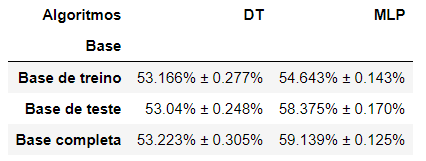
\includegraphics[width=\linewidth]{figures/resultados}
    \caption{Média e desvio padrão da acurácia total para cada algoritmo. Fonte: acervo próprio.}
    \label{fig:resultados}
\end{figure}

De modo geral, tem-se que a árvore de decisão construída seguiu o padrão do \texttt{scikit-learn}, diferenciando-se desse por possuir profundidade máxima igual a 3 e utilizar as 10 características melhor correlacionadas de acordo com o \textit{ANOVA F-value}. Quanto à rede neural, ela também seguiu o padrão do \texttt{scikit-learn}, diferenciando-se desse por possuir o número de neurônios da camada oculta como sendo \textit{(número de entradas + número de saídas) / 2} e utilizar as 30 características melhor correlacionadas de acordo com o \textit{ANOVA F-value}. A rede neural construída pode ser vista na \autoref{fig:ann}.

Sendo assim, tem-se que a rede neural possui a seguinte arquitetura: 3 camadas (1 de entrada, com 30 neurônios; 1 oculta, com 15 neurônios; e 1 de saída, com 1 neurônio); função de ativação Unidade Linear Retificada; otimizador baseado em gradiente estocástico \textit{Adam} para ajustar os pesos; e taxa de aprendizagem constante. Mais informações da arquitetura estão na documentação do \href{https://scikit-learn.org/stable/modules/generated sklearn.neural_network.MLPClassifier.html}{\texttt{MLPClassifier}}.

\begin{figure}[t!]
    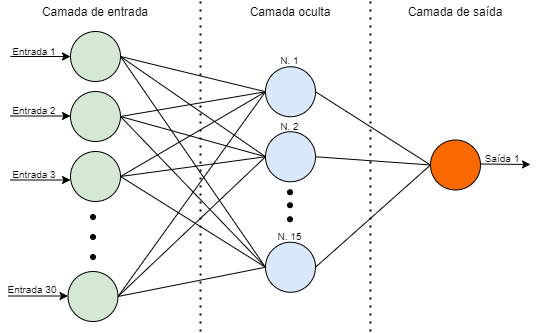
\includegraphics[width=\linewidth]{figures/ann}
    \caption{Arquitetura da rede neural utilizada. Fonte: acervo próprio.}
    \label{fig:ann}
\end{figure}

\section{Análise comparativa}\label{sec:analise}

Com os resultados expostos acima, mais especificamente na \autoref{fig:resultados}, podemos observar como os dois algoritmos apesentam acurácia semelhante para ambas baes de treino e de teste, sendo que a rede neural utilizada chegou a apresentar resultados melhores para a base de treino. Assim, podemos desconsiderar a ideia do \textit{overfitting} do nosso modelo, e apontar a validade de seus resultados.

Além disso, ao fazer análise da tabela completa com as métricas de cada execução presente em \textbf{\href{https://github.com/ygarasab/data-classification}{@ygarasab/data-classification}}, nos deparamos com uma alta sensibilidade em nossa árvore de decisão, o que demonstra a eficiência da mesma na determinação de seus nós, e refletindo a decisão anterior de redução da profundidade.

Por fim, voltando-se para os resultados, nota-se que a acurácia de teste dos algoritmos de árvore de decisão e rede neural não superaram em muito o modelo \textit{baseline} criado. Além disso, as acurácias de ambos os algoritmos são relativamente similares.  Considerando que o tempo de treinamento da rede neural é consideravelmente maior do que o da árvore de decisão, tem-se que o melhor algoritmo em geral para lidar com o conjunto de dados selecionado é a árvore de decisão. 

\section{Conclusão}\label{sec:conclusao}


Tendo em mente o exposto, cabe mencionar que outras técnicas poderiam ser testadas na tentativa de melhorar a acurácia, como substituir a seleção de características por extração de características através de técnicas de redução de dimensionalidade \textit{embedding-based}. Apesar disso, considerando as informações contidas no conjunto de dados analisado e com base no que se sabe acerca do contexto do problema, tem-se que o maior problema é a falta de informações mais relevantes e decisivas acerca da partida, como a quantidade de ouro coletada, mortes, abates, assistências, tempo de partida, entre outros. 

Assim, ressalta-se que a ferramenta GitHub foi utilizada como sistema de versionamento no decorrer do desenvolvimento deste trabalho, de forma que as contribuições dos integrantes desta equipe possam ser registradas e vistas. Neste repositório encontra-se um arquivo \texttt{.ipynb} (i.e., um Jupyter Notebook) informando de maneira mais detalhada o tratamento da base de dados, a seleção de atributos, a aplicação dos algoritmos e os resultados obtidos. Todas essas contribuições adicionais podem ser encontradas em \textbf{\href{https://github.com/ygarasab/data-classification}{@ygarasab/data-classification}}.


\bibliographystyle{sbc}
\bibliography{sbc-template}

\end{document}
